\documentclass{article}

% Language setting
% Replace `english' with e.g. `spanish' to change the document language
\usepackage[english]{babel}

% Set page size and margins
% Replace `letterpaper' with `a4paper' for UK/EU standard size
\usepackage[letterpaper,top=2cm,bottom=2cm,left=3cm,right=3cm,marginparwidth=1.75cm]{geometry}
\usepackage{biblatex}
\addbibresource{references.bib}

% Useful packages
\usepackage{amsmath}
\usepackage{graphicx}
\usepackage{csquotes}
\usepackage[colorlinks=true, allcolors=blue]{hyperref}
\DeclareMathOperator{\Var}{Var}
\DeclareMathOperator{\E}{E}
\DeclareMathOperator{\Prob}{Prob}
\DeclareMathOperator{\drift}{drift}


\title{Quantitative Models for Options Pricing}
\author{Fabian Farestam, typeset by Om Gupta}
\date{September 2022}

\begin{document}
\maketitle

\section{Introduction}

This document is an overview of quantitative models for option pricing to be implemented in OpenBBTerminal. When learning about options pricing, I recommend you to start with learning the Cox-Ross-Rubinstein Binomial model, then Black-Scholes model and later on advance to more complicated models. \\
Note that none of this is my (Fabian Farestam’s) research. It’s just a reformulation and a collection of material from multiple sources.

\section{Cox-Ross-Rubinstein Binomial Model}

The binomial pricing model \cite{cox} has a simple concept, namely that it builds a tree of possible pricing with a certain amount of steps until the time of the options maturity and calculates the arbitrage free price based on this tree. It’s easy to implement (can be $O(2^{n}$)) and also very practical while clearly demonstrating the no arbitrage argument. In special limiting cases of this we can get both the Black-Scholes model as well as the Cox-Ross jump process model (similar to the hybrid jump diffusion model by Merton). \\
The model assumes that:

\begin{itemize}
    \item The stock price follows a multiplicative binominal process over discrete periods
    \item The interest rate is constant and one might borrow and lend as much as wished at this interest rate. (For convenience we assume that $r > 1$)
\end{itemize}

\subsection{Notation}
\begin{itemize}
    \item $u$: Asset return with the probability of $q$ 
    \item $d$: Asset return with the probability of $1 - q$
    \item $S$: Stock Price
    \item $q$: Probability of tree path taken
    \item $r$: Riskless interest rate
    \item $C$: Value of a call option
    \item $K$: Strike Price
\end{itemize}

\subsection{One Step Tree}
The setup is simple, the stock returns over each period is either $u - 1$ with the probability of $q$, or $d - 1$ with the probability $1 - q$. Thus the price at the end of the period will be $uS$ or $dS$. Note that the relation $u > r > d$ must always be held. An illustration of this is:

\begin{figure}
\centering
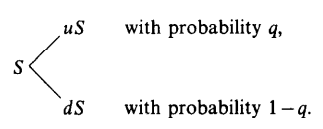
\includegraphics[width=0.3\textwidth]{one-step-tree.png}
\caption{\label{fig:onestep}Source: Cox, Ross, Rubinstein}
\end{figure}

To calculate the value of this simple setup, where there’s only one step, we use:
\begin{align*}
    C_{u} = \max(0, uS - K) \\
    C_{d} = \max(0, dS - K)
\end{align*}
When using a number of shares, $g$ (some use $\delta$ instead of g) and dollar invested in riskless bonds, $B$. Thus:
\begin{align*}
    C_{u} = g u S + r B \\
    C_{d} = g d S + r B 
\end{align*}
After solving for $g$ and $B$,
\begin{align}\label{eq:1}
    \begin{split}
    g = \frac{C_{u} - C_{d}}{(u - d)S} \\
    B = \frac{uC_{d} - dC_{u}}{(u - d)r}
    \end{split}
\end{align}
If no arbitrage exists then:
\begin{equation*}
    C = gS +B
\end{equation*}
Which then implies
\begin{equation}\label{eq:2}
    C = \frac{p C_{u} + (1 - p) C_{d}}{r}
\end{equation}
where $p=\frac{r-d}{u-d}$ and $1-p=\frac{u-r}{u-d}$ \\ [5ex]
From \ref{eq:2} we can make three observations:
\begin{enumerate}
    \item $q$ is not used, thus even if investors have different opinions about the probabilities they can still agree to this relationship! ($p$ is $q$ if investors were to be risk neutral)
    \item Investor’s risk attitude doesn’t matter.
    \item The stock price is the only random variable.
\end{enumerate}
\subsection{Two Step Tree}
For a two step tree we get the following structure:\\
\begin{figure}
\centering
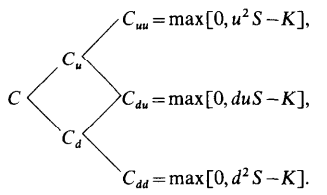
\includegraphics[width=0.3\textwidth]{two_step_tree.png}
\caption{\label{fig:twostep}Source: Cox, Ross, Rubinstein}
\end{figure}
To this new tree we adapt \ref{eq:2}
\begin{align}\label{eq:3}
    \begin{split}
    C_{u} = \frac{p C_{uu} + (1-p) C_{ud}}{r} \\
    C_{d} = \frac{p C_{du} + (1-p) C_{dd}}{r}
    \end{split}
\end{align}
We don't need to change \ref{eq:1}  but just we need to adjust our hedge portfolio with the new values gotten from \ref{eq:3} \\
So to get the value of the call we substitute \ref{eq:3} into \ref{eq:2}, which results in:
\begin{align}\label{eq:4}
    \begin{split}
    C & = \frac{p^{2} C_{uu} + 2 p (1 - p)  C_{ud} + (1 - p)^{2}  C_{dd}}{r} \\
    & = \frac{p^{2}*\max(0, u^{2}S - K) + 2 p (1 - p) * \max(0, duS - K)}{r}
    \end{split}
\end{align}
From this we conclude that all assumptions made from \ref{eq:2} also hold for \ref{eq:4}. Now the list of variables that determine $C$ is $S, K, n, u, d$ and $r$.
\subsection{Binomial tree with any amount of steps}
We can find the call value recursively, by starting at the expiration and working backwards, for any amount of steps:
\begin{equation}\label{eq:5}
    C = \frac{\sum_{j=0}^{n}{n \choose j} p^{j}(1-p)^{n-j}\max(0, u^{j}d^{n-j}S - K)}{r^{n}}
\end{equation}
We’re not yet done since we can express this in a way nicer form by some transformations:
\begin{equation}\label{eq:6}
    C = \frac{\sum_{j=a}^{n} {n \choose j} p^{j}(1-p)^{n-j} (u^{j}d^{n-j}S - K)}{r^{n}}
\end{equation}
where $a$ (represents minimum stock upwards moves for finishing in the money) is the smallest non negative larger greater than $\frac{\log(K / S d^{n})}{\log(u / d)} $ \\
We'll break up the above formula into two terms:
\begin{equation}\label{eq:7}
    C = S *\frac{\sum_{j=a}^{n} {n \choose j} p^{j}(1-p)^{n-j} (u^{j}d^{n-j})}{r^{n}} - K * \frac{\sum_{j=a}^{n} {n \choose j} p^{j}(1-p)^{n-j}}{r^{n}}
\end{equation}
In formula \ref{eq:7} we have two brackets, when taking a closer look at them one realises that we can express them as complementary binomial distribution function $\phi$. We can sum this up as the final simple Binomial Pricing formula:
\begin{equation}\label{eq:8}
    C = S *\phi(a; n, p') - K r^{-n} * \phi(a; n, p)
\end{equation}
where $p=\frac{r-d}{u-d}$ and $p'=\frac{u}{r}p$\\ [2ex]
Natural values for $u$ and $d$ are $u = e^{\sigma \Delta t}$ and $d=\frac{1}{u}=e^{-\sigma \Delta t}$ where $\sigma$ represents the volatility of the asset under consideration \\ [2ex]
Note that the formula above is only valid for American non-dividend paying call options.
\subsection{Dividends}
In this part in order to account for the dividend we assume that the stock has a constant dividend yield, $\delta$ on the ex-dividend date and a total of $v$ ex-dividend days. To account for dividend we need to define $\rho$ as one plus the interest rate over a period of $h=\frac{t}{n}$. The total return  is $\rho^{n} = r^{t}$, and we can express $\rho= r^{\frac{t}{n}}$. \\
A major difference in this model “extension“ is that early exercise is optimal in some cases. Early exercise is in fact optimal when $S > S^{*}$, where $S^{*}$ is the “critical” price of the stock where the following equation holds:
\begin{equation}\label{eq:9}
    S^{*} - K = \frac{p*C(n,i-1,j+1) + (1-p)*C(n,i-1,j)}{\rho}
\end{equation}
for $j = 0, 1, 2, .., n-i$ where $C(n, i, j) =$ call value $n-i$ periods from now, $S^{*} = u^{j}d^{n-i-j}(1-\delta)^{v(n,1)}*S$, and $v(n,i)=\sum_{k=1}^{n-1}v_{k}$ \\ [4ex]
From \ref{eq:9}, we get 
\begin{equation}\label{eq:10}
   C(n,i,j) = \max\left(u^{j}d^{n-i-j}(1-\delta)^{v(n,1)}*S - K, \frac{p*C(n,i-1,j+1) + (1-p)*C(n,i-1,j)}{\rho}\right)
\end{equation}
Important to note is that here we traverse the price the binomial tree recursively, thus starting with $i = 0$ and ending with $i = n$. We apply the previous results into the calculations of the previous ones. \\ [2ex]
The hedge ratio of the portfolio is:
\begin{equation*}
    g = \frac{C(n, n - 1, 1) - C(n, n -1, 0)}{(u - d) * S}
\end{equation*}
\subsection{Limiting Cases: Black-Scholes + Cox-Ross jump process}
We’ll start exploring these limiting cases by splitting our steps into small pieces. By setting $h$, the time elapsed between each step, as $h = \frac{t}{n}$. Now to get to a continuous tree we simply set $n \rightarrow \infty$. Again, we have $\rho^{n} = r^{t}$ so that $\rho = r^{\frac{t}{n}}$\\ [2ex]
From here we need to express $u$ and $d$ in terms of $n$. There’s two ways, one results in the Black Scholes model and the other in the Cox-Ross jump process model.
\subsubsection{Black-Scholes}
We’ll express the returns $u$ and $d$ from here on as $\log u$ and $\log u$, so over multiple periods we get that the final stock return is:
\begin{equation}\label{eq:11}
    \log (\frac{S^{*}}{S}) =  j \log u + (n - j) * \log d = j \log \left(\frac{u}{d}\right) + n \log d
\end{equation}
$j$ is the random number of upwards moves, which occurred during $n$ periods. We can now express the expected return and the return variance:
\begin{align*}
    \E[\log (\frac{S^{*}}{S})] &= \log \left(\frac{u}{d}\right)*\E[j] + n \log d \\
    \Var[\log (\frac{S^{*}}{S})]& = (\log \left(\frac{u}{d}\right))^{2}*\Var[j]
\end{align*}
Since $\E[j] = n q$; and $\Var[j] = n q (1 - q)$; (due to the variance of one period being: $q(1-q)^{2} + (1-q)(0 - q)^{2} = q(1-q))$. Now we simplify the formulas above:
\begin{gather}
\begin{split}
    \E\left[\log \left(\frac{S^{*}}{S}\right)\right] = (\log \left(\frac{u}{d}\right)q +\log d)*n  = \mu n \\
    \Var\left[\log \left(\frac{S^{*}}{S}\right)\right] = (\log \left(\frac{u}{d}\right))^{2}q(1-q)*n = \sigma n
\end{split}
\end{gather}
Now we need to adjust $u$ and $d$ so that we get realistic results. Below $\overline{\mu}$ and $\overline{\sigma}$ are the empirical values of $\mu$ and $\sigma$ to so we get the empirical values after adjusting $u$ and $d$. \\ [3ex]
As $n \rightarrow \infty$ :
\begin{gather*}
    (\log \left(\frac{u}{d}\right)q +\log d)*n \rightarrow \overline{\mu}n \\
    (\log \left(\frac{u}{d}\right))^{2}q(1-q)*n \rightarrow \overline{\sigma} n
\end{gather*}
Thus, 
\begin{gather}
\begin{split}
    u = \exp\left(\overline{\sigma}h^{\frac{1}{2}}\right) \\
    d = \exp\left(-\overline{\sigma}h^{\frac{1}{2}}\right) \\
    q = \frac{1+\frac{\overline{\sigma}}{\overline{\mu}}\left(\frac{n}{t}\right)^{\frac{1}{2}}}{2}
\end{split}
\end{gather}
This makes that every probability and possible outcome get changed. Now we use the central limit theorem, when applied it to our problem, says that as $n \rightarrow \infty$, if \ref{eq:14} below holds then \ref{eq:15} applies, where $N(z)$ is the standard normal distribution:
\begin{align} \label{eq:14}
    \frac{q|\log u - \mu|^{3} + (1-q)|\log d - \mu|^{3}}{\sigma^{3}n^{\frac{1}{2}}} & \rightarrow 0 \\
    \Prob\left[\frac{\log\left(\frac{S^{*}}{S}\right) - \mu n}{\sigma n^{\frac{1}{2}}} \le z\right] & \rightarrow N(z) \label{eq:15}
\end{align}
When we rewrite the Black Scholes theorem in terms of the the previously used notation, we get:
\begin{equation}
   C =  S N(x) - K r^{-t} N(x - \sigma t^{\frac{1}{2}})
\end{equation}
where $x = \frac{\log\left(\frac{S}{Kr^{-t}}\right)}{\sigma t^{\frac{1}{2}}} + \frac{\sigma t^{\frac{1}{2}}}{2}$
\subsubsection{Cox Ross Jump Process}
To get the Cox-Ross jump process model, we set $u$, $d$, and $q$ to the following values:
\begin{gather*}
    u = u \\
    d = \exp\left(\zeta \left(\frac{t}{n}\right)\right) \\
    q = \lambda \left(\frac{t}{n}\right) \\
\end{gather*}
where $\lambda$ is the intensity function (or rate) of the underlying Poisson process and $\zeta$ is related to the intensity measure of the distribution.\\
The central limit theorem no longer holds for these values and the stock price converges to a log-Poisson distribution as $n \rightarrow \infty$. This complementary Poisson distribution can be expressed in the following form:
\begin{equation}
    \psi (x,y) = \sum_{i=x}^{\infty} \frac{e^{-y}y^{i}}{i!}
\end{equation}
This allows the Cox-Ross jump process model to be written as:
\begin{equation}
    C = S \psi(x,y) - Kr^{-t} \psi\left(x,\frac{y}{u}\right)
\end{equation}
where $y=\frac{(\log r - \xi) u t }{u-1}$ and $x$ is the the smallest non-negative integer greater than $\frac{\log\left(\frac{K}{S}\right)}{\log u}$
\section{Black-Scholes Model}
\subsection{Notation}
\begin{itemize}
    \item $S_{t}$: Price of underlying asset at time $t$
    \item $\mu$: Annualized drift rate of $S$
    \item $\sigma$: Standard deviation of the asset's log returns
    \item $\phi (m,s)$: Normal distribution with mean $m$ and standard deviation of $s$
    \item $\eta$: Continuously compounded rate of return
    \item $U$: Annualized annual expected return in period $\Delta t$
    \item $V$: Annualized annual expected return expressed in a compounding frequency of $\Delta t$ over a longer period of time
    \item $\epsilon$: random from the standard normal distribution $\phi(0, 1)$
    \item $r$: Annual risk-free rate of interest
    \item $f$: Price of derivative
\end{itemize}
\subsection{Assumptions}
These assumptions are used to derive the Black-Scholes-Merton \cite{hull} differential equation and the equation only holds in this theoretical environment. Note that some of these assumptions can and will be accounted for at a later stage of the document. For instance interest rates can be stochastic, thus relaxing the conditions assumed.
\begin{itemize}
    \item Random walk - Asset prices follow geometric Brownian motion: 
    \begin{equation*}
        dS = \mu S dt + \sigma S dz
    \end{equation*}
    \item Lognormal distributions - this results in that the price at time T corresponds to: 
    \begin{equation} \label{eq:19}
        \ln S_{T} \sim \phi\left(\ln S_{0} + \left(\mu - \frac{\sigma^{2}}{2}\right)T, \sigma T^{\frac{1}{2}}\right)
    \end{equation}
    \item Non dividend (will later show dividend extension)
    \item Market:
    \begin{itemize}
        \item No arbitrage
        \item Lend and borrow
        \item Buy and short
        \item No transaction fees
        \item Continuous security trading
    \end{itemize}
    \item $\mu$, $r$, and $\sigma$ are constant
    \item $r$ is the same for all maturities
\end{itemize}
\subsection{Calculations}
If we start with the normal distribution of returns we get that the expected value of $S_{T}$, $\E[S_{T}]$: 
\begin{equation*}
    \E[S_{T}] = S_{0} e^{\mu T}
\end{equation*}
and variance of $S_{T}$:
\begin{equation*}
    \Var[S_{T}] = S_{0}^{2} e^{2\mu T}[e^{\sigma^{2}T}-1]
\end{equation*}
\subsubsection{Rate of Return}
Further using the log normal properties of the price at time $T$ we get: 
\begin{equation*}
    S_{T} = S_{0} e^{\eta T}
\end{equation*}
and it follows that 
\begin{equation} \label{eq:20}
    \eta = \frac{1}{T} \ln\left(\frac{S_{T}}{S_{0}}\right)
\end{equation}
For correctly understanding \ref{eq:20} we need to get $\ln\left(\frac{S_{T}}{S_{0}}\right))$, we get this when transforming \ref{eq:19}: 
\begin{equation}\label{eq:21}
    \ln\left(\frac{S_{T}}{S_{0}}\right) \sim \phi\left(\left(\mu - \frac{\sigma^{2}}{2}\right)T, \sigma T^{\frac{1}{2}}\right)
\end{equation}
So it then follows that 
\begin{equation} \label{eq:22}
    \eta = \left(\mu - \frac{\sigma^{2}}{2}, \frac{\sigma} {T^{\frac{1}{2}}}\right)
\end{equation}
Now we can define $V$ (expected return over a longer period of time) from \ref{eq:22}, which results in:
\begin{equation} \label{eq:23}
    V = \mu - \frac{\sigma^{2}}{2}
\end{equation}
In order to compare it to $U$ and properly understand it, we express geometric Brownian motion in discrete-time:
\begin{equation} \label{eq:24}
    \frac{\Delta S}{S} = \mu \Delta t + \sigma \epsilon (\Delta t)^{\frac{1}{2}}
\end{equation}
$U$ is then naturally:
\begin{equation} \label{eq:25}
    U = \mu \Delta t
\end{equation}
\subsubsection{Volatility}
Further drawing from \ref{eq:24} we get that as $\Delta t$ approaches zero, we can see that $\sigma (\Delta t)^{\frac{1}{2}}$ is approximately equal to the standard deviation of proportional change in asset price in $\Delta t$ \\ [2ex]
In equation \ref{eq:20} “the volatility of a stock price can be defined as the standard deviation of the return provided by the stock in one year when the return is expressed using continuous compounding“ (citation from John C. Hull see sources).\\ [2ex]
While in \ref{eq:19} we see that vol (volatility) is also the stdev (standard deviation) of the natural logarithmic asset price  at the end of one year.
\subsubsection{Ito's Lemma}
The price of any derivate is a function of stochastic variables of the derivative underlying and time, thus we need to understand some of the behaviour of functions of stochastic variables, known as Ito’s lemma. The value of a variable x follows an Ito process:
\begin{equation} \label{eq:26}
    dx = a(x, t) dt + b(x, t) dz
\end{equation}
Here $a$ and $b$ are functions of $x$ and $t$ and $dz$ is a Wiener process. The drift rate of $x$ is thus $a$ and the variance of $x$ is $b^{2}$. \\ [2ex]
What Ito’s lemma says is essentially that a function, G, of x and t, where dz is the same Wiener process as above in \ref{eq:26}, follows an Ito process:
\begin{equation} \label{eq:27}
    dG = \left[\frac{\partial G }{\partial x} a + \frac{\partial G }{\partial t} + \frac{1}{2}\frac{\partial^{2} G }{\partial x^{2}} * b^{2}\right]dt + \frac{\partial G }{\partial x} b dz
\end{equation}
Thus, the drift rate is 
\begin{equation} \label{eq:28}
    \drift(G) = \frac{\partial G }{\partial x} a + \frac{\partial G }{\partial t} + \frac{1}{2}\frac{\partial^{2} G }{\partial x^{2}} * b^{2}
\end{equation}
and the variance
\begin{equation} \label{eq:29}
    \Var[G] = (\frac{\partial G }{\partial x} b)^{2}
\end{equation}
Now from Ito’s lemma we can set $a = \mu S$ , $b = \sigma S$ and $x = S$ into \ref{eq:27}:
\begin{equation} \label{eq:30}
    dG = \left[\frac{\partial G }{\partial S} \mu S + \frac{\partial G }{\partial t} + \frac{1}{2}\frac{\partial^{2} G }{\partial S^{2}} * \sigma^{2} S^{2}\right]dt + \frac{\partial G }{\partial S} \sigma S dz
\end{equation}
(Note that the source of uncertainty dz affects both S and G)
\subsubsection{Derivation of the Black-Scholes-Merton differential equation}
Since $f$ is the price of the derivate on S, $f$must be a function of $S$ and $t$. Now we’ll use formula \ref{eq:30} with respect to $f$ rather than $G$:
\begin{equation} \label{eq:31}
    df = \left[\frac{\partial f }{\partial S} \mu S + \frac{\partial f }{\partial t} + \frac{1}{2}\frac{\partial^{2} f }{\partial S^{2}} * \sigma^{2} S^{2}\right]dt + \frac{\partial f }{\partial S} \sigma S dz
\end{equation}
or in discrete form (note \ref{eq:24})
\begin{equation} \label{eq:32}
    \Delta f = \left[\frac{\partial f }{\partial S} \mu S + \frac{\partial f }{\partial t} + \frac{1}{2}\frac{\partial^{2} f }{\partial S^{2}} * \sigma^{2} S^{2}\right]\Delta t + \frac{\partial f }{\partial S} \sigma S \Delta z
\end{equation}
In the discrete form of the Brownian process, 
\begin{equation}\label{eq:33}
        \Delta S = \mu S \Delta t + \sigma S \Delta z
    \end{equation}
As mentioned in the section about Ito’s lemma, \ref{eq:26} and \ref{eq:27} have the same Wiener process, thus we get that $f$ and $S$ follow the same Wiener process! We can therefore say $\Delta z = \sigma \epsilon (\Delta t)^{\frac{1}{2}}$ see \ref{eq:24} in the formulas \ref{eq:32} and \ref{eq:33} are the same! \\ [2ex]
Hull describes it the best here:
\begin{displayquote}
It follows that by choosing a portfolio of stock and the derivate, the Wiener process can be eliminated. The appropriate portfolio is: \\
-1: derivate\\
$\frac{\partial f }{\partial S} $ : Shares\\ [2ex]
The holder of this portfolio is short one derivate and long an amount of $\frac{\partial f }{\partial S}$ of shares.
\end{displayquote}
So we define $\Pi$ as the portfolio value, thus:
\begin{equation}\label{eq:34}
\begin{split}
    \Pi = -f + \frac{\partial f }{\partial S} S \\
    \Delta \Pi = -\Delta f + \frac{\partial f }{\partial S} \Delta S
\end{split}
\end{equation}
Since we assume that there is no arbitrage $\Delta z$ must be 0, since the portfolio must be riskless during $\Delta t$ and earn the risk-free rate (otherwise there would be arbitrage). It follows that:
\begin{equation}\label{eq:35}
    \Delta \Pi = r \Pi \Delta t
\end{equation}
When we plug \ref{eq:32} and \ref{eq:33} in \ref{eq:34}, we get
\begin{equation}\label{eq:36}
    \Delta \Pi = - \left[\frac{\partial f }{\partial t} - \frac{1}{2}\frac{\partial^{2} f }{\partial S^{2}} * \sigma^{2} S^{2}\right] \Delta t
\end{equation}
Using \ref{eq:35} and \ref{eq:36}, we get 
\begin{equation}\label{eq:37}
    \frac{\partial f }{\partial t} + r S \frac{\partial f}{\partial S} +\frac{1}{2}\frac{\partial^{2} f }{\partial S^{2}} * \sigma^{2} S^{2} - rf = 0
\end{equation}\\
Finally we have arrived to the Black-Scholes-Merton differential equation!\\[3ex]
The BSM differential equation is riskless for a infinitesimally small time period ($lim_{\Delta t\to\ 0}$). Since $S$ and $t$ changes, $\frac{\partial f}{\partial S}$ changes as well, so the ratio between stocks and derivatives kept in the portfolio gets rebalanced. \\[2ex]
The particular derivative depends on the boundary conditions that are used. Different boundary condition results in different derivatives. For instance for European call options you need to use the following boundary conditions at $t=T$:
\begin{equation*}
    f = \max (S - K, 0)
\end{equation*}
or for an European put option, it is:
\begin{equation*}
    f = \max (K - S, 0)
\end{equation*}
\subsection{Pricing Formulas}
\subsubsection{European options}
We get the formulas for European options by solving the BSM differential equation for the previously mentioned boundaries (where $c$ for call and $p$ for put is used):
\begin{align}
    \begin{split} \label{eq:38}
        c &= S_{0}N(d1) - X e^{-rT} N(d2) \\ 
        p &= X e^{-rT} N(-d2) - S_{0} N(-d1)
    \end{split}
\end{align}
where 
\begin{gather*}
        d_{1} = \frac{\ln\left(\frac{S_{0}}{K}\right)+\left(r^{2}+\frac{\sigma^{2}}{2}\right)T}{\sigma T^{\frac{1}{2}}} \\
        d_{2} = \frac{\ln\left(\frac{S_{0}}{K}\right)+\left(r^{2}-\frac{\sigma^{2}}{2}\right)T}{\sigma T^{\frac{1}{2}}} = d_{1} - \sigma T^{\frac{1}{2}}
\end{gather*}
The input for dividend paying European options has to be adjusted, which is covered in the Appendix
\subsubsection{American call options with non-dividend paying stocks}
American call option on a stock that pays no dividends during the life of the option will not be exercised early and, hence, can be valued as a European option with the standard Black-Scholes formula.
\subsubsection{European warrants issued by firm on its own stocks}
\begin{equation}
    W = \left[\left(S_{0} + \frac{M}{N}W\right)N(d_{1}) - Ke^{-rT}N(d_{2})\right]\frac{N\gamma}{N + M\gamma}
\end{equation}
where 
\begin{itemize}
    \item $\gamma$ : The amount of shares per warrant
    \item $N$ : Outstanding shares
    \item $M$ : Outstanding European warrants
\end{itemize}
\subsection{Modelling Input}
\subsubsection{Estimating volatility}
If we define
\begin{itemize}
    \item $n+1$ : Observations
    \item $\tau$ : Time in years
    \item $u_{i}$ : Continuously compounded return in i\emph{th} interval
\end{itemize}
Due to $S_{i}= S_{i-1} e^{ui}$,
\begin{equation}
    u_{i} = \ln \left(\frac{S_{i}}{S_{i-1}}\right)
\end{equation}
To then calculate the deviations from the mean we use a similair calculation as with the standard deviation:
\begin{equation*}
    s = \left(\frac{1}{n-1} \sum_{i=1}^{n}u_{i}^{2} - \frac{1}{n(n-1)}\left(\sum_{i=1}^{n}u_{i}\right)^{2}\right)^\frac{1}{2}
\end{equation*}
Now, we see from \ref{eq:19} that $\sigma  = \frac{s}{\tau^{\frac{1}{2}}}$ but this has some flaws so the standard error can be shown to be
\begin{equation}
    \alpha = \frac{\sigma }{(2n)^{0.5}}
\end{equation}
Note that the volatility has to be annualised since the time used is in years.
Choosing n is hard, so here is the general recommendation from Hull:
\begin{displayquote}
Choosing an appropriate value for n is not easy. Ceteris paribus, more data generally leads to more accuracy. However, $\sigma$ does change over time and data that are too old may not be relevant for predicting the future. A compromise that seems to work reasonably well is to use closing prices from daily data over the most recent 90 to 180 days. An often used rule of thumb is to set the time period over which the volatility is measured equal to time period over which it is applied.
\end{displayquote}
GARCH can also be used, see the GARCH Models in volatility models. \\
If the stock pays dividend, we just need to change $u_{i}$ during a time interval that includes an ex-dividend day, given by:
\begin{equation}
    u_{i} = \ln \left(\frac{S_{i}+D}{S_{i-1}}\right)
\end{equation}
where $D$ is the dividend amount
\section{Merton's Jump-Diffusion Model}
The Jump-Diffusion model \cite{Kou_2007} \cite{mert} assumes that underlaying asset follows a jump-diffusion process. The downside from this is that it requires two more input parameters, which are “hard” to observe in the market. The parameters are the following:
\begin{itemize}
    \item $\lambda$ : Expected number of jumps per year
    \item $\gamma$ : Percentage of total volatility explained by the jumps
\end{itemize}
The JmpDif (Jump-Diffusion model) solves the problem with the “Mes Mile-effect“ that comes with the BSM model. It also doesn’t assume the log normal distribution. Prices of assets vary in “normal“ vibrations in price, for example due to temporary supply and demand imbalances, and in “abnormal“ vibrations, caused by asset/sector specific news (for example quarterly reports). The “normal“ vibrations can be modelled by geometric Brownian motion and the “abnormal“ by a “jump“ process.
\subsection{Additional Notation}
\begin{itemize}
    \item $a$: Instantaneous expected asset return
    \item $\epsilon$: Expectations operator
    \item $k$: Percent change of asset price if event occurs
    \item $W$: Options price
    \item $P$: Portfolio value
    \item $\tau$: Time to expiry
    \item $E$: Exercise price
\end{itemize}
\subsection{Calculations}
\subsubsection{Poisson-driven Process}
To start to describe the above mentioned “jump“ process, we’ll use a “Poisson-driven“ process. We now look at the probability of an event occurring in this Poisson distributed process:
\begin{enumerate}
    \item $\Prob$[event doesn't occurs in time interval $(t, t+h)$] = $1- \lambda h + O(h)$
    \item $\Prob$[event occurs once in time interval $(t, t+h)$] = $\lambda h + O(h)$
    \item $\Prob$[event occurs multiple times in time interval $(t, t+h)$] = $O(h)$
\end{enumerate}
Above, we can set $h$ to whatever we want. $O(h)$ is the asymptotic order symbol defined by $\psi(h) = O(h)$ when $\lim_{h\to 0} \left[\frac{\psi(h)}{O(h)}\right] = 0.$ $\lambda$ is the mean number of arrivals per time unit. \\ [2ex]
If this event occurs, then we draw Y from a distribution, so if we ignore the continuity we would get something like $S(t+h) = S(t) Y$ \\ 
The stock price can be expressed stochastically as:
\begin{equation}\label{eq:43}
    \frac{dS}{S} = (a - \lambda k) dt + \sigma dz + dq
\end{equation}
In the formula above $\sigma^{2}$ is the variance at the moment (if no Poisson event occurs), dz is the standard Gauss-Wiener process and $q(t)$ is the Poisson process of the event described above. k is defined as $\epsilon(Y - 1)$, where $(Y- I)$ is the random variable percentage change in the stock price if the Poisson event occurs. \\ [2ex]
To make it clear, \ref{eq:43} can be rewritten as:
\begin{equation*}
    \frac{dS}{S} = (a - \lambda k) dt + \sigma dz
\end{equation*}
if event doesn't occur and
\begin{equation*}
    \frac{dS}{S} = (a - \lambda k) dt + \sigma dz + (Y-1)
\end{equation*}
if event does occur\\
Setting a, $\lambda$, k and $\sigma$ to constants, then the random ratio of stock price at time 0 and time $t$ is:
\begin{equation}
    \frac{S_{t}}{S_{0}} = \exp \left(a - \frac{\sigma^{2}}{2} - \lambda k t + \sigma z(t)\right) Y(n)
\end{equation}
$z(t)$ is a Gaussian random variable, which has a mean of 0 and variance of $t$. $Y(n)$ is defined as:
\begin{equation}
    Y(n) = \begin{cases} 1 \text{ , if } n=0 \\
    \Pi_{j=1}^{n} Y_{j} \text{ , if } n\geq1
    \end{cases}
\end{equation}\label{eq:46}
$Y_{j}$ are independently and identically distributed and $n$ is Poisson distributed with parameter $\lambda t$.
Now, we apply \ref{eq:43} to the options price, $W$, where $W(t) = F(S, t)$
\begin{equation}
    \frac{dW}{W} = (a_{W} - \lambda  k_{W}) dt + \sigma_{W} dz + dq_{W}
\end{equation}
It has the same terminology as \ref{eq:43} but everything is for the option \\ [2ex]
When applying Ito’s lemma to the continuous part and a similar to the Poisson process we get:
\begin{equation}\label{eq:47}
\begin{gathered}
    a_{W} = \frac{\frac{\sigma^{2}}{2}S^{2}F''_{SS}(S,t) + (a-\lambda k) S F'_{S} + F'_{t} + \lambda \epsilon (F(S,Y,t) - F(S,t))}{F(S,t)}\\
    \sigma _{W} = \frac{F'_{S}(S,t) \sigma S}{F(S,t)}
\end{gathered}
\end{equation}
Since $q_{W}(t)$ is dependent on $q(t)$ (so only if $q(t)$ occurs $q_{W}(t)$ occurs). If the event manifests $Y = y$ and $Y_{W} = \frac{F(SY, t)}{F(S, t)}$. This is how we partly get the result in \ref{eq:47}. \\[2ex]
Let’s try to model portfolio value similarly to \ref{eq:43} and \ref{eq:46}, where $w{1}$, $w_{2}$, and $w_{3}$ will be the proportions of stock, option and riskless asset:
\begin{equation}
    \frac{dP}{P} = (a_{P} - \lambda  k_{P}) dt + \sigma_{P} dz + dq_{P}
\end{equation}
Based on \ref{eq:43} and \ref{eq:46} we get ($w_{3} = 1 - w_{1} - w_{2}$ has been substituted) formulas similar to \ref{eq:47}, but notice the differences and similarities:
\begin{equation} \label{eq:49}
    \begin{gathered}
    a_{P} = w_{1}(a - r) + w_{2}(a_{W} -r) + r \\
    \sigma_{p} = w_{1}\sigma + w_{2}\sigma_{W} \\
    Y_{P} - 1 = w_{1}(Y - 1) +  w_{2}\frac{F(SY, t) - F(S, t)}{ F(S, t) }
    \end{gathered}
\end{equation}
Due to portfolio mixing being a linear operation and the option price being a non-linear function of the stock price, we can’t use the simple method with assumptions we used to get the BSM differential equation (see appendix for greater detail).
\subsubsection{Getting a options pricing formula}
When the Black Scholes “no arbitrage“ method cannot be used, we can still derive a options formula if we can figure of the options expected return as a function of the stock price and time to expiry. We define the function of $g(S, \tau $to be the equilibrium momentary expected return. We’ll use this and \ref{eq:47}, we get that $F$ (a function of $\tau$ this time) must hold the following equation (which is a bit similar to the BSM):
\begin{equation} \label{eq:50}
    \frac{1}{2}\sigma^{2}S^{2}F''_{SS} + (a - \lambda k)SF'_{S} - F'_{\tau} - g(S,\tau)F + \lambda \epsilon (F(S,Y,t) - F(S,t)) = 0
\end{equation}
subject to the boundary conditions $F(0, \tau) = 0$ and $F(S, 0) = \max(0, S - E)$ \\ [2ex]
The equation of \ref{eq:50} can be solved, but then you have to know $a$ and $g(S, \tau)$. However this is a bit hard and a not so fruitful approach. \\
Now we’ll try price it with CAPM (Capital Asset Pricing Model), which BSM also assumed to be true. Here the jumps will represent non-systematic risks and this is the only source of uncertainty. Thus the $\beta$ of the portfolio must be 0 and in CAPM the expected return of such portfolios (with 0 $\beta$) must be $r$ ($a_{P^{*}} = r$). Here follows from \ref{eq:49} $w_{1}^{*}(a - r) + w_{2}^{*}(a_{w} -r) = 0$ and we substitute $w_{1}^{*}$ \& $w_{2}^{*}$:
\begin{equation} \label{eq:51}
    \frac{a-r}{\sigma} = \frac{a_{W}-r}{\sigma_{W}}
\end{equation}
When using \ref{eq:51}, \ref{eq:47} we get that $F$ must hold the following equation:
\begin{equation} \label{eq:52}
    \frac{1}{2}\sigma^{2}S^{2}F''_{SS} + (r - \lambda k)SF'_{S} - F'_{\tau} - rF + \lambda \epsilon (F(S,Y,t) - F(S,t)) = 0
\end{equation}
\ref{eq:52} still depends on the boundaries specified before and the same equation, except that we have replaced $a \& g(S, \tau)$ with $r$.
\subsubsection{Solution to the equation}
To solve the equation \ref{eq:52} and obtain a solution, we have to further specify the distribution of $Y$, a partial solution. We’ll start by defining $W(S, \tau; E, r, \sigma^2) $as the no jump Black Scholes formula:
\begin{equation}\label{eq:53}
    W(S, \tau; E, r, \sigma^2) = S \phi (d_{1}) - E e^{-r\tau} \phi(d_{2})
\end{equation}
where $\phi(y) = \frac{1}{(2\pi)^{\frac{1}{2}}}\int_{-\infty}^{y}\exp\left({-\frac{s^{2}}{2}}\right)\,ds$ i.e. the cumulative normal distribution function
and 
\begin{gather*}
    d_{1} = \frac{\ln\left(\frac{S}{E}\right)+\left(r+\frac{\sigma^{2}}{2}\right)\tau}{\sigma \tau^{\frac{1}{2}}} \\
    d_{2} = d_{1} - \sigma \tau^{\frac{1}{2}}
\end{gather*}
Defining the random variable $X_{n}$ to have the same distribution as the product of $n$ independently and identically distributed random variables, with the same distribution of $Y$ used in \ref{eq:43}, where $X_{0} = 1$. $\epsilon_{n}$ is the expectation operator over the distribution of $X_{n}$. The solution to \ref{eq:52} for the options price when the current stock price is S can be written as:
\begin{equation} \label{eq:54}
    F(S, \tau) = \sum_{n=0}^{\infty} e^{-\lambda \tau}\frac{(\lambda \tau)^{n}}{n!} \left[\epsilon_{n} W(SX_{n}e^{-\lambda \tau}, \tau; E, \sigma^2, r) \right]
\end{equation}
\subsection{Special cases of the pricing formula}
In these special cases formula \ref{eq:54} can be vastly simplified. Case number 1 is when the Poisson event occurs, the stock price goes to zero and case number 2 is when $Y$ has a log-normal distribution.
\subsubsection{Case 1}
We need to set $Y = 0$ with a probability to one if the event occurs, $X_{n}$ = 0 if $n \neq= 0$ and $k = -1$. Then \ref{eq:54} can be written as:
\begin{equation}
    F(S, \tau) =  e^{-\lambda \tau}\left[W(Se^{\lambda \tau}, \tau; E, \sigma^2, r) \right] = W(S, \tau; E, \sigma^2, r + \lambda)
\end{equation}
It is identical to the standard Black Scholes, but the interest rate is $r' = r + \lambda$
\subsubsection{Case 2}
If $Y$ is log-normally distributed, $\gamma = \log (k + 1)$ and $\sigma^{2}$ is the variance of the logarithm of $Y$. $X_{n}$ has a log-normal distribution of which $\sigma^2 n$ is the variance of $\log X_{n}$ and $\epsilon_{0}(X_{0}) = e^{n\gamma}$
\begin{equation}
    f_{n}(S, \tau) = W(S, \tau; E, v_{n}^2, r_{n})
\end{equation}
where $v_{n}^2 = \sigma^2 + \frac{n\sigma^{2}}{\tau}$ and $r_{n} = r - \lambda k + \frac{n\gamma}{\tau}$ \\[2ex]
It is the standard Black Scholes option, where $v_{n}^{2}$ is the “formal“ stocks variance per unit time and $r_{n}$ is the “formal” instantaneous rate of interest. Finally we have:
\begin{equation}
    F(S, \tau) = \sum_{n=1}^{\infty} e^{-\lambda \tau} \frac{(\lambda(1+k)\tau)^{n}}{n!}f_{n}(S,\tau)
\end{equation}
What happens in these “magic“ formulas is that $f_{n}$ is the value of the options when we know how many Poisson jumps will occur during the options life time. $F(S, \tau)$, the actual value of the option, is the weighted sum of these prices, where the weight responds to the probability that a Poisson random variable (with characteristic parameter $\lambda(1+k)\tau$) will take the value of $n$.
\section{Heston Model}
The Heston model \cite{Heston_1993} is a stochastic volatility model, thus it has one Stochastic Differential Equation (SDE) for the asset and another SDE for the stochastic volatility.
\subsection{Calculations}
\subsubsection{Volatility Modelling}
In the Heston model we assume that the stock price follows:
\begin{equation}
    dS = \mu S dt + v^{\frac{1}{2}}Sdz_{1}
\end{equation}
If the volatility, $v$, follows an Ornstein-Uhlenbeck process:
\begin{equation}
    dv^{\frac{1}{2}} = -\beta v^{\frac{1}{2}} dt + \sigma dz_{2}
\end{equation}
Then by using Ito’s lemma we see that the variance $v$ follows:
\begin{equation} \label{eq:60}
    dv = (\sigma ^{2} - 2\beta v)dt + 2 \sigma v^{\frac{1}{2}}dz_{2}
\end{equation}
\ref{eq:60} can be rewritten as the square-root process and as in CIR:
\begin{equation}
    dv = K(\theta - v) dt + \sigma v^{\frac{1}{2}} dz_{2}
\end{equation}
$z_{1}$ and $z_{2}$ have the correlation of $\rho$. We assume a constant interest rate $r$. The price of the asset $f(S, v, t)$ must hold \ref{eq:62}, to follow the no arbitrage argument:
\begin{equation} \label{eq:62}
    \frac{1}{2}vS^{2}\frac{\partial^{2} f}{\partial S^{2}} + \rho \sigma v S \frac{\partial^{2} f}{\partial S \partial v} + \frac{1}{2}v\sigma^{2}\frac{\partial^{2} f}{\partial v^{2}} + r S \frac{\partial f}{\partial S} + [K(\theta - v) - \lambda] \frac{\partial f}{\partial v} - rf + \frac{\partial f}{\partial t} = 0
\end{equation}
In \ref{eq:62} $\lambda$ represents the price of volatility risk and is asset independent.  Research suggests that $\lambda$ is non zero for equity options; there’s approaches to model it for consumption assets but we won’t consider them here. We use the following boundary conditions for a European call option with the strike X and with T as maturity in \ref{eq:62}: 
\begin{equation} \label{eq:63}
    \begin{gathered}
    f(S, v, T) = \max(S - X, 0) \\ 
    U(0, v, t) = 0 \\
    \frac{\partial f}{\partial S} (\infty, v, t) = 1 \\
    f (S, \infty, t ) = S \\ 
    r S \frac{\partial f}{\partial S} (S, 0, t) + K \theta \frac{\partial f}{\partial v} (S, 0, t) - r f(S, 0, t) + \frac{\partial f}{\partial t} (S, 0, t) = 0
    \end{gathered}
\end{equation}
From similarity with the Black Scholes formula, we guess that our solution will be along the lines of:
\begin{equation} \label{eq:64}
     C(S, v, t) = SP_{1} - XP(t, T)P_{2}
\end{equation}
where $SP1$ is the present value of spot price in optimal exercise and $XP(t, T)P2$ is the present value of strike price payment
We plug \ref{eq:64} into \ref{eq:63} and $P_{1}$ and $P_{2}$ must satisfy \ref{eq:65} below
\begin{equation} \label{eq:65}
    \frac{1}{2}v\frac{\partial^{2} P_{j}}{\partial x^{2}} + \rho \sigma v \frac{\partial^{2} P_{j}}{\partial x \partial v} + \frac{1}{2}v\sigma^{2}\frac{\partial^{2} P_{j}}{\partial v^{2}} + (r + u_{j} v) \frac{\partial P_{j}}{\partial x} + [a-b_{j}v] \frac{\partial P_{j}}{\partial v} + \frac{\partial P_{j}}{\partial t} = 0
\end{equation}
for $j=1,2$ and where we have 
\begin{equation*}
   \begin{gathered}
   x=\ln S \\
   u_{1} = \frac{1}{2} \\
   u_{2} = -\frac{1}{2} \\
   a = K\theta \\ 
   b_{1} = K + \lambda - \rho \sigma \\ 
   b_{2} = K + \lambda
   \end{gathered}
\end{equation*}
Since \ref{eq:65} must follow \ref{eq:62}, we have the terminal condition
\begin{equation}\label{eq:66}
    P_{j}(x, v, T; \ln(X)) = 1_{(x \geq \ln(X))}
\end{equation}
From this formula we get that the probabilities are risk-neutralized. The conditional probability, $P_{j}$, of the option expiring ITM is
\begin{equation} \label{eq:67}
    P_{j}(x, v, T; \ln(X)) = \Prob[x(T) \geq \ln(X)\, | \,x(t) = x, v(t) = v]
\end{equation}
\ref{eq:67} holds when x follows
\begin{equation}
    \begin{gathered}
    dx(t) = (r + u_{j} v) dt + v(t)^{\frac{1}{2}} dz_{1}(t) \\
    dv = (a_{j} - b_{j} v) dt + \sigma v(t)^{\frac{1}{2}} dz_{2}(t)
    \end{gathered}
\end{equation}
\subsection{Characteristics}
Since there’s no closed form solution to the probability from \ref{eq:67}, we have to calculate the characteristic functions. At time $T$ in the future, $f(x, v, t)$ is the expectation of a function $g(x(T), v(T))$, where $x(t)$ and $v(t)$ follow the risk neutral process from \ref{eq:66}:
\begin{equation}
    f(x, v, t) = \E[g(x(T), v(T)) \,|\, x(t) = x, v(t) = v]
\end{equation}
We apply Ito's lemma to this:
\begin{equation} \label{eq:70}
    df = \left[\frac{1}{2}v\frac{\partial^{2} f}{\partial x^{2}} + \rho \sigma v \frac{\partial^{2} f}{\partial x \partial v} + \frac{1}{2}v\sigma^{2}\frac{\partial^{2} f}{\partial v^{2}} + (r + u_{j} v) \frac{\partial f}{\partial x} + [a-b_{j}v] \frac{\partial f}{\partial v} + \frac{\partial f}{\partial t}\right] dt + [r + u_{j} v] \frac{\partial f}{\partial x}dz_{1} + [a-b_{j}v] \frac{\partial f}{\partial v} dz_{2}
\end{equation}
$\E[df]=0$ and when we apply this knowledge to \ref{eq:70}, we get 
\begin{equation}\label{eq:71}
    \frac{1}{2}v\frac{\partial^{2} f}{\partial x^{2}} + \rho \sigma v \frac{\partial^{2} f}{\partial x \partial v} + \frac{1}{2}v\sigma^{2}\frac{\partial^{2} f}{\partial v^{2}} + (r + u_{j} v) \frac{\partial f}{\partial x} + [a-b_{j}v] \frac{\partial f}{\partial v} + \frac{\partial f}{\partial t} = 0
\end{equation}
\ref{eq:71} is called the Fokker-Planck forward equation and is very useful, since we know that:
\begin{equation}
    f(x, v, T) = g(x, v)
\end{equation}
Due to this we can set $g(x, v)$ equal to some function and then solve $f(x, v, T)$ from it. Let’s take a look at some examples:
\begin{itemize}
    \item $g(x, v) = \delta(x - x0) \rightarrow$  Conditional probability density that $x(T) = x_{0}$ at time $t$.
    \item $g(x,v) = 1_{(x \geq \ln(X))} \rightarrow$ Conditional probability that $x(T) > \ln(K)$ at time $t$.
    \item $g(x,v) = e^{i\phi x} \rightarrow$ Characteristic functions
\end{itemize}
To solve for the characteristic functions (which are the solution to the last example of $g(v, x)$ above) we have to have an idea on the functional form. By using the linearity of \ref{eq:70} coefficients, we guess:
\begin{equation} \label{eq:73}
    f(x, v, t) = \exp[C (T - t) + D (T - t) v + i\phi x]
\end{equation}
In order to reduce the functional form to two ordinary differential equations, we plug \ref{eq:73} into \ref{eq:70}:
\begin{gather}
    -\frac{1}{2}  \sigma^{2} \phi^{2} + \rho \sigma \phi i D + \frac{1}{2} D^{2} + u_{j} \phi i - b_{j} D + \frac{\partial D}{\partial t} = 0 \\
    r \phi i + a D + \frac{\partial C}{\partial t} = 0
\end{gather}
subject to $C(0) = 0$ and $D(0) = 0$
\subsection{Result}
To summarize we previously get that the characteristic functions of \ref{eq:66} which hold the terminal condition $f_{j}(x, v, T; \phi) = e^{i \phi x}$ satisfy \ref{eq:62}. The final solution of the characteristic function is:
\begin{equation}\label{eq:76}
    f_{j}(x, v, t; \phi) = \exp(C(T - t; \phi) + D(T - t; \phi) v + i \phi x);
\end{equation}
where 
\begin{equation}
    \begin{gathered}
    C(\tau, \phi) = r \phi i \tau + \frac{a}{\sigma^{2}} * {(b_{j} - \rho \sigma \phi i + d) \tau - 2 \ln\left[\frac{1 - g ed r}{1 - g}\right]} \\
    D(\tau,\phi) = \frac{(b_{j} - \rho \sigma \phi i + d)} {\sigma^{2}} \frac{1 - e^{d r}} {1 - g e^{d r}} \\
    g = \frac{b_{j} - \rho \sigma \phi i + d}{b_{j} - \rho \sigma \phi i - d} \\
    d = (\rho \sigma \phi i - b_{j})^{2} - \sigma^{2} (2 u_{j} \phi i + \phi^{2})
    \end{gathered}
\end{equation}
If we want the probabilities, we can invert the characteristic functions:
\begin{equation}\label{eq:78}
     P_{j}(x, v, T; \ln(X)) = \frac{1}{2} + \frac{1}{\pi} \int_{0}^{\infty} \Re\left[\frac{e^{-i \phi \ln(X)} f_{j}(x, v, T; \phi)}{i \phi}\right] \, d\phi
\end{equation}
If we want to get the price of a European call option, then we have to get the solution from \ref{eq:64}, \ref{eq:76} and \ref{eq:78}.
\subsection{Modelling Input}
Heston recommends the following default parameter values for the simulation of option prices: \ref{tab:tab1}\newline\newline
\begin{table}[]
    \centering
    \begin{tabular}{c|c}
     \textbf{Parameter} & \textbf{Value} \\
    Mean reversion & $K^{*}=2$ \\
    Long-run variance & $\theta^{*}=0.01$ \\
    Current variance & $v(t) = 0.01$ \\
    Correlation of $z_{1}(t)$ and $z_{2}(t)$ & $\rho = 0.0$ \\
    Volatility & $\sigma = 0.1$ \\
    Option maturity & $\tau = 0.5$ years\\
    Interest rate & $r=0$ \\
    Strike Price & $X=100$ \\
    \end{tabular}
    \caption{Default parameters for use with the Heston Model}
    \label{tab:tab1}
\end{table}
Note that you need to adjust (at least) some of these to get realistic results, for instance the strike price, X and the options maturity.  
\printbibliography

\clearpage
\pagenumbering{roman}
\appendix
\section{Cox-Ross-Rubinstein Binomial Model}

\subsection{Modelling a known dollar dividend}
The binomial tree gets a bit more complicated when the dividend, D, is fixed, but this is often a partly reasonable assumption (i.e. a firm allocates a certain amount of money for dividends → when the stock price suddenly doubles the dividend does not often). See Figure \ref{fig:divtree}.\\
\begin{figure}
\centering
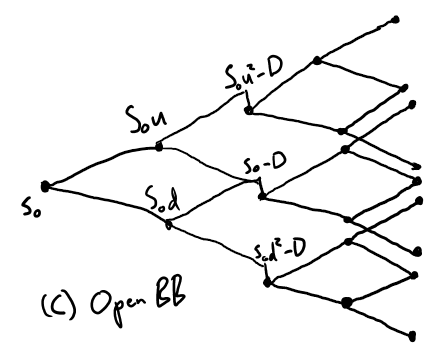
\includegraphics[width=0.3\textwidth]{five-step-tree-w-dividend.png}
\caption{\label{fig:divtree} Binomial tree with known dividend}
\end{figure}
Before the ex-dividend date the Stock price is simply $S_0 u^j d^n - j$ (for $j = 0, 1, 2, …,$ until dividend), then the stock price becomes $S_0 u^j d^n - j - D$ on the step after the ex-dividend date and after this point in time the stock price is $(S_0 u^j d^{n - j} - D) * u^k d^l$ (where k and l are steps up and down after the dividend). For the evaluation we start at $n = 0$ and go across the tree and value the options value at each step as usual, but with the adjusted stock prices.\\This quickly becomes a very processing power heavy computation as we add more dividend dates, since for each ex-dividend date at time, $b$, we have to simulate $n^b$ new binomial trees in parallel. In order to avoid this for European we can discount the value of the dividend.

\subsection{Proof of convergence}
We can write the binomial options pricing theorem \ref{eq:8} as:
\begin{equation}\label{eq:A2.1}
    C = S *\phi(a; n, p') - K \rho^{-n} * \phi(a; n, p)
\end{equation}
The only drastic difference is that $\rho^{-n}$ is here instead of $r{-t}$ but they’re equal to each other. Thus we only need to prove the following:
\begin{equation}\label{eq:A2.2a}
    \phi(a; n, p') \to N(x)
\end{equation}
\begin{equation}\label{eq:A2.2b}
    \phi(a; n, p) \to N(x - \sigma t^{0.5})
\end{equation}
If we manage to prove \ref{eq:A2.2a} we just need the same process for proving \ref{eq:A2.2b}, which we’ll skip.

$\phi(a; n, p)$ is the sum of n random variables, which takes on $1$ (with the probability of $p$) or $0$ (with the probability of $p - 1$), this will be greater than or equal to $a$ (recall that it is the smallest non-negative integer greater than $\frac{\log(\frac{K}{S} d^n)}{\log(\frac{u}{d}))}$. $j$, the random value of the sum, has the mean $n p$ and the standard deviation $\sqrt{n p (1 - p)}$, thus:
\begin{equation}\label{eq:A2.3}
    1 - \phi(a; n, p) = Prob[j \le a - 1] = Prob\left[\frac{j - n p}{\sqrt{n p (1 - p)}} \le \frac{a - 1 - n p}{\sqrt{n p (1 - p)}}\right]
\end{equation}

We need to modify \ref{eq:A2.2a} and \ref{eq:A2.2b}, since we now consider a stock, where \ref{eq:11} holds, with the probability p instead of q:
\begin{gather}
    \sigma_p^2 = p (1 - p) [\log(\frac{u}{d})]^2 \\
    \mu_p = p \log(\frac{u}{d}) + \log d 
\end{gather}
Using $\sigma_p, \mu_p$ and formula \ref{eq:11}, we get \ref{eq:15} and can set the following:
\begin{equation}\label{eq:A2.4}
    \frac{j - n p}{\sqrt{n p (1 - p)}} = \frac{\log(S^* / S) - \mu_p n}{\sigma_p n^{0.5}}
\end{equation}
From previously we can define $a - 1$ as:
\begin{equation}
    a - 1 = \frac{\log(K / S d^n)}{\log(\frac{u}{d})} - \epsilon = \frac{\frac{\log(\frac{K}{S})}{n \log(d)}}{\log(\frac{u}{d})} - \epsilon
\end{equation}
Using the formula from above we create the following equality from \ref{eq:A2.3}:
\begin{equation}\label{eq:A2.5}
    \frac{a - 1 - n p}{\sqrt{n p (1 - p)}} = \frac{\log(\frac{K}{S}) - \mu_p n - \epsilon \log(\frac{u}{d})}{\sigma_p n^{0.5}}
\end{equation}
Now we can use \ref{eq:A2.4} and \ref{eq:A2.5} to express \ref{eq:A2.3} as:
\begin{equation}\label{eq:A2.6}
    1 - \phi(a; n, p) = Prob\left[\frac{\log(\frac{S^*}{S}) - \mu_p n}{\sigma_p n^{0.5}} \le \frac{\log(\frac{K}{S}) - \mu_p n - \epsilon \log(\frac{u}{d})}{\sigma_p n^{0.5}}\right]
\end{equation}
The central limit theorem can now be applied to \ref{eq:A2.6}. Thus if \ref{eq:A2.7a} holds, which it does due to \ref{eq:A2.7b}, then we can use the central limit theorem to get \ref{eq:A2.7c}:\\

As $n \rightarrow \inf$:\begin{gather}
    \frac{p |\log u - \mu_p|^3 + (1 - p)|\log d - \mu_p|^3}{\sigma_p n^{0.5}} = \frac{(1 - p)^2 + p^2}{n p (1 - p)^{0.5}} \rightarrow 0\label{eq:A2.7a}\\
    p \rightarrow \frac{1}{2} + \frac{1}{2}\frac{\log r - \frac{1}{2}\sigma^2}{\sigma}\sqrt{\frac{t}{n}}\label{eq:A2.7b}\\
    1 - \phi(a; n, p) \rightarrow N(z) = N\left(\frac{\log{\frac{K r^{-t}}{S}}}{\sigma t^{0.5}} + \frac{1}{2} \sigma t^{0.5}\right)\label{eq:A2.7c}
\end{gather}
From the result of \ref{eq:A2.7c} we evaluate $\mu_p n$, $\sigma_p^2n$ and $\log{\frac{u}{d}}$ as $n \rightarrow \inf$. This results in $\mu_p n \rightarrow (\log r - \frac{1}{2}\sigma^2) * t$, $\sigma_p^2n \rightarrow \sigma t^{0.5}$ and $\log{\frac{u}{d}} \rightarrow 0$. (Something surprising is that $p \not= q$ and therefore $mu_p \not= \mu$ and $\sigma_p \not= \sigma$)

Since $1 - N(z) = N(-z)$, we can conclude the proof of convergence with:
\begin{equation}\label{eq:A2.8}
    \phi(a; n, p) \rightarrow N(-z) = N\left(\frac{\log{\frac{S}{k r^{-t}}}}{\sigma t^{0.5}} - \frac{1}{2} \sigma\right) = N(x - \sigma t^{0.5})
\end{equation}

\section{Black-Scholes Model}

\subsection{Applying Ito's lemma to the $\ln$ of the stock price}
Note: This is only here for context and for those who want to understand BSM at a bit more fundamental level.\newline

Previously we used formula \ref{eq:19} and here we'll see how we can get there by applying Ito's lemma to derive the process followed by $\ln S$. So we set:
\begin{equation}
    G = \ln S
\end{equation}
Now we calculate partial derivatives of $G$:
\begin{gather}
    \frac{\partial G}{\partial S} = \frac{1}{S}\\
    \frac{\partial^2 G}{\partial^2 S} = -\frac{1}{S^2}\\
    \frac{\partial G}{\partial t} = 0
\end{gather}
By putting the results from the partial derivatives of G into \ref{eq:30}, we obtain:
\begin{equation}\label{eq:B1.1}
    dG = (\mu - \frac{\sigma^2}{2}) dt + \sigma dz
\end{equation}
The result implies that $G$ follows a Wiener process, which is generalized. Naturally it's drift rate is:
\begin{equation}
    \mu - \frac{\sigma^2}{2}
\end{equation}
and its variance:
\begin{equation}
    \sigma^2
\end{equation}
This might be interesting, but it truly becomes handy when we want to observe the change in G between time zero and a future time $T$. Due to it being normally distributed, we get that the mean at time $T$ is:
\begin{equation}
    (\mu - \frac{\sigma^2}{2}) T
\end{equation}
and it's variance at time $T$ is:
\begin{equation}
    \sigma^2 T
\end{equation}
Thus we get from \ref{eq:B1.1} and our knowledge of the nature of G that the difference between $S_0$ and $S_T$ is:
\begin{equation}
    \ln S_T - \ln S_0 ~ \phi\left((\mu - \frac{\sigma^2}{2}) T, \sigma^2 T\right)
\end{equation}
which can be rewritten in the form (this is the same as \ref{eq:21}):
\begin{equation}
    \ln{\frac{S_T}{S_0}} ~ \phi\left((\mu - \frac{\sigma^2}{2}) T, \sigma^2 T\right)
\end{equation}
By applying Ito's lemma to $G = \ln S$, we derived formula \ref{eq:21}, which we easily can change into \ref{eq:19}. I hope that this is sufficient and helps to understand the BSM better.

\subsection{Differential equation for stock price with known dividend yield}
If the stock pays a dividend $q$, we have that $\mu = r - q$ otherwise there wouldn't be risk neutrality. We follow the same process (with Ito's lemma and the set up of the portfolio) mentioned above until after formula \ref{eq:36}. The portfolio holder earns capital equal to $\Delta\Pi$ and dividends on the stock, which equals to:
\begin{equation}\label{eq:B2.1}
    q S \frac{\partial f}{\partial S} * \Delta t
\end{equation}
We now use \ref{eq:B2.1} to define $\delta W$, the portfolio holders change in wealth during time $\delta t$:
\begin{equation}\label{eq:B2.2}
    \Delta W = \left[-\frac{\partial f}{\partial t} - \frac{\partial^2 f}{2 \partial S^2} * \sigma^2 S^2 + q S \frac{\partial f}{\partial S} \right] \Delta t
\end{equation}
The equation \ref{eq:B2.2} essentially responds to \ref{eq:36} $+$ \ref{eq:B2.1}. So we conclude that \ref{eq:35} doesn't hold in this particular case, since $\Delta W$ is our "new" $\Delta \Pi$:
\begin{equation}\label{eq:B2.3}
    \Delta W = r \Pi \Delta t
\end{equation}
Now we see that plugging \ref{eq:B2.2} and (the first formula in) \ref{eq:34} into \ref{eq:B2.3} results in the following:
\begin{equation}
    \left[-\frac{\partial f}{\partial t} - \frac{\partial^2 f}{2 \partial S^2} * \sigma^2 S^2 + q S \frac{\partial f}{\partial S} \right] \Delta t = r \left(-f + \frac{\partial f}{\partial S} * S\right) \Delta t
\end{equation}
Simplifying to:
\begin{equation}\label{eq:B2.4}
    \frac{\partial f}{\partial t} + (r - q) S * \frac{\partial f}{\partial S} + \frac{1}{2} \sigma^2 S^2 \frac{\partial^2 f}{2 \partial S^2} = r f
\end{equation}
See the similarity between \ref{eq:B2.4} and \ref{eq:37}.

\subsection{Adjust input parameters to handle dividends}
The stock price of a firm can be split into two parts, a riskless component and a risky component (the rest). When the option has matured, all dividend will have been payed and this riskless component won't exist any longer, thus it doesn't affect the volatility. Therefore we just need to discount the stock price by the sum of the present value of all dividends payed during the options life time. Thus in "pseudo" math, we have: \newline\newline
$S_0 = P - \sum d_i e^{t_i r}$, where $d_i = i$:th dividend amount and $t_i = $ Time until $d_i$ is paid\newline\newline
After this we just need to calculate \ref{eq:38} to get the value of a European dividend paying call/put option.

\subsection{Derivation of pricing formula for European warrants issued by firm on its own stock}
The firm has $M$ outstanding European warrants and $N$ outstanding shares. Due to the share dilution caused by warrants we have after exercise $N + M \gamma$, where $\gamma$ is the amount of shares per warrant. The firms equoty also increases after exercise to $V_T + M \gamma X$, where company equity, including warrants at time $T$ is $V_T$. Thus the share price directly after exercise becomes:
\begin{equation}
    \frac{V_T + M \gamma X}{N + M \gamma}
\end{equation}
The warrant pay off if it is exercised corresponds to:
\begin{equation}
    \frac{N \gamma}{N + M \gamma} * \max\left(\frac{V_T}{N} - X, 0\right)
\end{equation}
From this we conclude:
\begin{equation}
    V_0 = S_0 + \frac{M W}{N}
\end{equation}
Now we just have to plug everything into \ref{eq:38}

\section{Merton's Jump-Diffusion Model}
\subsection{Applying the Black Scholes method to Merton's Jump-Diffusion Model}
When trying to apply the Black Scholes analysis to the portfolio we have to set $\lambda = 0$ (thus setting $dq = dq_w = 0$) and the portfolio return could be made by picking $W_1 = w_1^{*}$ and $w_2 = w_2^{*}$ so that $w_1 \sigma + w_2 \sigma_w = 0$. Then the returns must be equal to $r$, the risk free rate. Using these assumptions we conclude with the help of formula \ref{eq:49}:
\begin{equation}
    \frac{a - r}{\sigma} = \frac{a_w - r}{\sigma_w}
\end{equation}
With the equation above and (the first equality of) \ref{eq:47} with $\lambda = 0$, we arrive at the Black Scholes differential equation:
\begin{equation}
    \frac{1}{2} \sigma^2 S^2 F''_{SS} + r S F'_S - r F + F'_t
\end{equation}
Important to note is that this does however *not* hold when $\lambda \not= 0$, due to the jump process. From the last equation in \ref{eq:49} we can conclude that there are no portfolio weights ($w_1$, $w_2$) that could eliminate the jump risk. Thus if $Y$ has positive dispersion, then for any $w_1$ and $w_2$, $Y_p - 1$ will take on non-zero values for some possible values of $Y$. Trying to sue the Black Scholes hedge also won't work due to this formula already being continuous in time.\\
We can try to find the return characteristics with the Black Scholes hedge, this portfolio $P^{*}$ will be the following:\\
\newline If the Poisson process doesn't occur:
\begin{equation}
    \frac{dP^{*}}{P^{*}} = (a_p^{*} - \lambda k_p^{*}) dt
\end{equation}
If the Poisson process doesn't occur:
\begin{equation}
    \frac{dP^{*}}{P^{*}} = (a_p^{*} - \lambda k_p^{*}) dt + Y_{p^{*}}
\end{equation}
\newline From this we can conclude that the portfolio price is predictable most of the time, except when once every $\frac{1}{\lambda}$ on average, where the portfolio value will jump. To further continue this route we use the second equation in \ref{eq:47} and the last equation in \ref{eq:49} to get:
\begin{equation}\label{eq:C1.1}
    Y_{p^{*}} - 1 = w_2 \frac{F(S Y, t) - F(S, t) - F'_S(S, t) (S Y - S)}{F(S, t)}
\end{equation}
The formula above gives by the strict convexity of the option price in the stock price that $F(S Y, t) - F(S, t) - F'_S(S, t) (S Y - S)$ is positive for every value of Y. So if $w_2^{*}$ is positive then $Y_{p^{*}}$ will be positive and the unanticipated return on the hedge will always be positive.\\
From this we can conclude that investors buy the stock and short the options will gain money on average, except for when a jump occurs and vice versa. This explains the nature of options, since most of them expire worthless and when they don't they often achieve great returns.

\subsection{Verifying that \ref{eq:54} is a solution to \ref{eq:52}}
In order to verify that \ref{eq:54} is a solution to \ref{eq:52} with the boundary conditions $F(0, \tau) = 0$ and $F(S, 0) = \max(0, S - E)$ (as mentioned under \ref{eq:50}), we'll rewrite \ref{eq:54}:
\begin{gather}
    F(S, \tau) = \sum_{n=0} ^{\infty} P_n(\tau) * \epsilon_n(W(V_n, \tau; E, \sigma^2, r))\\
    P_n(\tau) = e^{-\lambda \tau} \frac{(\lambda \tau)^n}{n!}\\
    V_n = S X_n e^{-\lambda \tau}
\end{gather}
Now we differentiate the formula above:
\begin{gather}
    S F'_S(S, \tau) = \sum_{n=0}^{\infty} P_n(\tau) \epsilon_n(V_n W_1) \label{eq:C2.1}\\
    S^2 F''_{SS}(S, \tau) = \sum_{n=0}^{\infty} P_n(\tau) \epsilon_n(V_n^2 W_{11}) \label{eq:C2.2}
\end{gather}
Continuing with:
\begin{equation}\label{eq:C2.3}
    F'_{\tau}(S, \tau) = - \lambda F - \lambda k \sum_{n=0}^{\infty} P_n(\tau) \epsilon_n(V_n W_1) + \sum_{n=0}^{\infty} P_n(\tau) \epsilon_n(W_2) + \lambda \sum_{n=1}^{\infty} \frac{(\lambda t)^{n-1} e^{-\lambda \tau}}{(n - 1)!} \epsilon_n(V_n W_2)
\end{equation}
We continue to simplify \ref{eq:C2.3} by substituting \ref{eq:C2.1} and setting m = n - 1
\begin{equation}\label{C2.3.1}
    F'_{\tau} = - \lambda F - \lambda k S F'_{S} + \sum_{n=0}^{\infty} P_n(\tau) \epsilon_n(W_2) + \lambda \sum_{m=0}^{\infty} P_m(\tau) \epsilon_{m+1}(W(V_{m+1}, \tau; E, \sigma^2, r))
\end{equation}
Finally we have the expression:
\begin{equation}\label{eq:C2.4}
    \epsilon_y(F(S, Y, \tau)) = \epsilon_y\left(\sum_{n=0}^{\infty} P_n(\tau) \epsilon_n(W(V_n Y, \tau; E, \sigma^2, r))\right)
\end{equation}
Which we can further simplify because of the definition of $X_n$, $X_{n+1}$ and $Y X_n$ are identically distributed and thus $\epsilon_y * \epsilon_n$ applied to $Y X_n$ is the same as $\epsilon_{n+1}$ applied to the same function $X_{n+1}$ substituted for $Y X_n$:
\begin{equation}\label{C2.4.1}
    \epsilon_y(F(S, Y, \tau)) = \sum_{n=0}^{\infty} P_n(\tau) \epsilon_{n+1}(W(V_{n+1} Y, \tau; E, \sigma^2, r))
\end{equation}
From the modified version of \ref{eq:54} (our first formula in the section) to \ref{C2.4.1}, we have:
\begin{multline}\label{eq:C2.5}
    \frac{1}{2} \sigma^2 S^2 F''_{SS} + (r - \lambda k) S F'_S - F'_{\tau} - r F =\\
    \sum_{n=0}^{\infty} P_n(\tau) \epsilon_n\left(\frac{1}{2} \sigma^2 V_n^2 W_{11} + r V_n W_1 - W_2 - r W\right) - \lambda k S F'_S + \lambda F + \lambda k S F'_S - \lambda \sum_{m=0}^{\infty} P_m(\tau) \epsilon_{m+1}(W(V_{m+1}, \tau; E, \sigma^2, r))\\
    = - \lambda(\epsilon_y(F(S Y, \tau) - F(S, \tau)))
\end{multline}
Since W satisfies the BSM differential equation, therefore for each $n$ we have:
\begin{equation}
    \frac{1}{2} \sigma^2 V_n^2 W_{11} + r V_n W_1 - W_2 - r W = 0
\end{equation}
From this follows that $F(S, \tau)$ satisfies \ref{eq:52}. For whatever $n$, $S = 0$ implies $V_n = 0$ and due to \ref{eq:53} we have $W(0, \tau: E, \sigma^2, r) = 0$ so the first boundary is satisfied (since $F(0, \tau) = 0$ in this case). \ref{eq:52} also gives:
\begin{equation}\label{eq:C2.6}
    \epsilon_n(W(V_n, 0; E, \sigma^2, r)) = \epsilon_n(\max(0, V_n - E)) \le \epsilon_n(V_n) = S(1 + k)^n
\end{equation}
Utilizing \ref{eq:C2.6}:
\begin{multline}\label{eq:C2.7}
    \lim{\tau \to 0} \sum_{n=1}^{\infty} P_n(\tau) \epsilon_n(W) \le \lim{\tau \to 0} \sum_{n=1}^{\infty} \frac{S e^{- \lambda \tau} [(1 + k)\lambda \tau]^n}{n!}\\
    = \lim{\tau \to 0} S e^{- \lambda \tau} (e^{(1+k)\lambda\tau}-1) \\
    = 0
\end{multline}
\ref{eq:C2.7} can then be used to prove that \ref{eq:54} satisfies the last bound $F(S, 0) = \max(0, S - E)$:
\begin{equation}\label{eq:C2.8}
    \lim{\tau \to 0} F(S, \tau) = \lim{\tau \to 0} P_0(\tau) \epsilon(W(V_0, \tau; E, \sigma^2, r)) = \max(0, S - E)
\end{equation}
\end{document}